\documentclass[review,number]{elsarticle}
\usepackage{algorithm2e}
\usepackage{graphics}
\usepackage{epsfig}
\usepackage{amsmath}
\usepackage{colortbl}
\usepackage{float}
\usepackage{graphicx}
\usepackage{rotating}

\begin{document}

\begin{frontmatter}

\title{A New Real-Time Traffic Sign Detection and Classification Method for Intelligent Vehicles}

\author[boun]{K.~Kaplan\corref{cor1}}
\ead{kaplanke@boun.edu.tr}
\author[boun]{C.~Kurtul}
\ead{caner.kurtul@gmail.com}
\author[boun]{H.~L.~Ak{\i}n}
\ead{akin@boun.edu.tr}
\cortext[cor1]{Corresponding author}
\address[boun]{Department of Computer Engineering, Bo{\u g}azi{\c c}i University,\\
34342, Bebek, \.{I}stanbul, Turkey.\\
Phone: +90 212 359 4523-24 \\
Fax: +90 212 287 2461}

\begin{abstract}
In this paper, a new real-time traffic sign detection and classification system with several contributions to improve the different phases of sign detection and classification is introduced. This work is a part of Automatic Driver Evaluation System (ADES) Project. The proposed system uses affine transformation coefficients as genetic algorithm parameters for sign detection. For the classification phase, the results show that neural networks are better than support vector machines for this specific application. The processing times and error rates show that this system can be used as a part of complex real-time applications. 
\end{abstract}

\begin{keyword}
Traffic Sign Detection and Classification, Affine Transformation, Genetic Algorithms, Radial Symmetry Check
\end{keyword}

\end{frontmatter}

\section{Introduction}
According to the Road Safety Action Program of European Commission ~\cite{signbib01}, more than one million accidents happen each year in Europe, causing more than 40000 deaths, nearly two million injuries, and an estimated indirect cost of 160 billion Euros, nearly two percent of the gross domestic product (GDP) of European Union. In addition to these statistics, the most noteworthy fact is that nearly all accidents are caused by driver mistakes.

With the advances in autonomous vehicles research, car manufacturers have started deploying more intelligence in their latest models. Parking assistance, adaptive cruise control, emergency brake assist, lane departure warning, and speed limit monitoring are among these new features appearing on the car market ~\cite{miscbib02, miscbib03}.  The main goal of such driver assistance and early warning systems is to reduce the number of accidents on the roads. However, the performance of such systems depends on their ability to recognize the conditions and the rules imposed by the traffic signs on the road the vehicle is cruising on. Therefore, one of the basic requirements for an intelligent vehicle is  having a fast and robust traffic sign detection method.

Even though such intelligent autonomous  vehicles are still under development and testing, these approaches can also be used in evaluating driver performance in real time to:

\begin{itemize}
    \item Assist drivers in driving more safely,
    \item Provide information about violations committed by the drivers to the traffic centrals,
    \item Automate of driver license examinations,
    \item Keep inventory of the traffic signs on highways,
    \item Provide supervision for the development of the autonomous urban driving systems.
\end{itemize}

This study is a part of the Automatic Driver Evaluation System (ADES) Project \cite{miscbib04}. The proposed system is designed for real-time detection, tracking, and classification of traffic signs from vision data. 

As discussed in Section \ref{sec:literature} there are various works already focused on identifying different kinds of traffic signs. However in this work, we not only focus on the accuracy but also the processing time of each frame so that we can spare additional time for the other stages of the proposed real time driver evaluation system.

We consider circular regulatory and triangular warning signs in Turkey.  Video captured in a car moving with varying speed in actual urban traffic with a wide range of lighting conditions such as sunny roads, dim lighted roads, shadows and even night-time driving conditions are processed. We used a novel Genetic Algorithm based method for the sign detection and tracking steps.  In the classification phase, we compared artificial neural networks (ANN) and support vector machines (SVM) for each traffic sign where the inputs are obtained by the classical occupancy grid feature extraction method.

The processing times and error rates show that this system can be used as a part of complex real-time applications.

The organization of the rest of the paper is as follows. In Section \ref{sec:literature} the existing sign detection and classification methods via analysis of visual data are discussed. The proposed approach is given in Section \ref{sec:pa}. Section \ref{sec:er} describes the experiments using video images captured under different light and weather conditions in real traffic, together with a discussion of the results. The conclusions are given in Section \ref{sec:conc}.

\section{Related Work}
\label{sec:literature}

A sign detection system can basically be decomposed into detection and classification steps. Researchers have proposed various techniques like Genetic Algorithms, Neural Networks, Kalman Filter, radial symmetry, Ada-Boost and LDA for these phases. The proposed Vision-based sign detection systems should be able to deal with adverse weather and lighting conditions.

\subsection{Neural Networks for Sign Classification}
One of the early studies on the topic is by Escalera \textit{et al} ~\cite{signbib02} in 1997. Detection is achieved by a shape analysis on a color threshold applied image, whereas classification is done by neural networks (NNs). Although hue-saturation-intensity (HSI) color space is invariant to lighting changes, red-green-blue (RGB) color space is preferred in this study. This is due to the fact that HSI formulation is nonlinear and therefore requires more processing power. The proposed approach applies a red-color threshold, followed by a corner detector for triangular signs and a circumference detector for circular signs. The detectors are basically a set of masks used for convolution. Two separate multilayer perceptron NNs have been trained for triangular and circular signs. The size of the input layer corresponds to an image of 30x30 pixels, and the output layer is of size ten, i.e., nine sign types plus one output that shows that the sign is not one of the nine. Ideal signs were used for training. 1620 training patters are created out of them by rotating, adding Gaussian noise, and displacing by 3 pixels.

Nguwi \textit{et al} ~\cite{nguwi08} also used multi-layer perceptron neural networks for both the detection and classification phases.

\subsection{Kalman Filters for Traffic Sign Detection and Tracking}
In ~\cite{Fang03} Fang \textit{et al} have additionally focused on the tracking of the signs through the image sequence. Prior to the tracking phase, they have used two NNs for detecting the signs: one for the color features and one for the shape features. A fuzzy approach is used to create an integration map of the shape and color features, which in turn is used to detect the signs. To reduce the complexity of the detection operations, the system can only detect signs of a particular size (8-pixel radius). Once the location of the sign is detected in the current frame, the size and location in the following frame is predicted by a Kalman filter. This significantly reduces the search space and increases the accuracy. Nevertheless, the detection technique proposed in this paper requires a large search space due to the complexity of the integration map.

Piccioli \textit{et al} ~\cite{signbib17} also incorporated both color and edge information to detect road signs from a single image. They applied Kalman-filter-based temporal integration of the extracted information for further improvement. They claimed that to improve the performance, their technique could be applied to temporal image sequences. In fact, the detection of road signs using only a single image has three problems: 1) to reduce the search space and time, the positions and sizes of road signs cannot be predicted; 2) it is difficult to correctly detect a road sign when temporary occlusion occurs; and 3) the correctness of road signs is hard to verify. By using a video sequence instead of temporal images, the information from the preceding images, such as the number of the road signs and their predicted sizes and positions can be preserved. This information can be used to increase the speed and the accuracy of road-sign detection in the subsequent images.

\subsection{Sign Detection Using AdaBoost and Haar Wavelet Features}
Bahlmann \textit{et al} ~\cite{Bahlmann05} suggest the use of AdaBoost ~\cite{miscbib13} and Haar wavelet \cite{miscbib14} features for detection, and a Gaussian probability density model for classification. Traditional object detection approaches generally apply color and shape detection separately one after the other. Regions that have falsely been rejected by color segmentation cannot be recovered in further processing. The main contribution of this paper, with this motivation, is a joint color and shape modeling within the AdaBoost framework. In addition, AdaBoost is mostly used to select gray-scale wavelet features specified by their position, width and height parameters. This study, on the other hand, requires wavelets to be applied on RGB images. Therefore, instead of gray-scale images, they have proposed a method to use RGB color images in the AdaBoost framework. The overall system is measured to perform with an error rate of 15 percent.

In ~\cite{baro09} Baro \textit{et al} also used an evolutionary version of Adaboost for detection and a tree structured discrete coding method for traffic sign classification.

\subsection{Matching Pursuit (MP) Algorithm for Traffic Sign Recognition}
Hsu and Huang ~\cite{signbib05} also use a two-fold approach for traffic signs: detection and recognition. The detection phase has three stages. In the first stage, a region where the road sign is more likely to be found is selected in the captured image. Here, either the color information or other heuristics (such as possible locations of road signs, geometrical characteristics of the signs) are used. In the second stage, the region of interest (ROI) is searched for finding the possible locations of the triangular or circular regions. Then, a closer view of the identified regions is captured by focusing the image. In the third stage, template-matching is applied to detect the road signs. In the recognition phase, MP filter ~\cite{signbib24} is used to recognize the road signs effectively. The MP algorithm uses a greedy heuristic to iteratively decompose any signal into a linear expansion of waveforms that are selected from a redundant dictionary of functions. Matching pursuits are general procedures to compute adaptive signal representations. The MP based recognition proposed in this paper is unfortunately too costly. While the computation time of the detection phase is 100 ms, the recognition operation using matching pursuit method requires about 250 ms.

\subsection{Support Vector Machine Approaches for Traffic Sign Detection and Classification}
A support vector machine (SVM) based study introduced by Maldonado-Bascon \textit{et al} ~\cite{Maldonadobascon07} can recognize circular, rectangular, triangular, and octagonal signs. They have used SVM for both detection and classification purposes. Linear SVMs are used as geometric shape classifiers at the detection phase. They operate on the color-segmented image (red, blue, yellow, white, or combinations of these colors). After color segmentation, \emph{blobs of interests} (BoI) are detected. Linear SVM executes on these blobs using the distance to borders (DtBs) as input vectors. For the sign classification phase, on the other hand, Gaussian-kernel SVMs are used. The input to the recognition stage is a block of 31x31 pixels in grayscale image for every candidate blob. The results show a high success rate and a very low amount of false detections in the final recognition stage. The results reveal that the proposed algorithm is invariant to translation, rotation, scale, and, in many situations, even to partial occlusions. This study does not suggest a tracking method. The overall recognition accuracy of the system is acceptable, and can detect different geometric shapes, i.e., circular, octagonal, triangular, and rectangular. However, it requires several performance enhancements in order to be applicable in real-time. The current computation time is 1.77 seconds per frame.

Another SVM-based solution by Kiran \textit{et al} ~\cite{signbib07} introduces an SVM Learning technique for traffic sign classification. Similar to many other studies, they have preferred color segmentation for detection. Only the hue and the saturation channels are used. Shape classification is performed using a linear support vector machine. Better shape classification performance is obtained by training the SVM using novel features called \textit{distance from center} (DfC) and \textit{distance to borders} (DtB). DfC is defined to be the distance from the center of the blob to the external edge of the blob, whereas, DtB is the distance from the external edge of the blob to its bounding box. Each segmented blob has four DtB vectors and four DfC vectors for left, right, top, and bottom directions. These vectors make the system invariant of translation, rotation and scale factors. Classification is evaluated both by using DtB alone, and also by combining DtB and DfC feature vectors. The proposed approach is more successful on circular signs than triangular ones. Also, using the joint features yielded slightly better results. The classification success rate is around 90 percent, and the true detection rate is around 96 percent.

In ~\cite{signbib09}, Jimenez \textit{et al} focus just on the sign detection problem, dividing it into two sub-blocks that perform shape classification and localization of the sign. This work is a successor of ~\cite{Maldonadobascon07} which used two different SVMs for detection and classification. The main contribution of this work is basically in the improvement of the detection block, where the new method developed here has proven to be more successful than the distance to borders (DtB) method, defined in their previous work ~\cite{Maldonadobascon07}. The classification of the shape is achieved by means of the connected components. Object rotations are handled with the use of the Fast Fourier Transform (FFT). The signature of each blob was used for the classification of the shape of the traffic sign. The normalization of the energy of the signature makes the algorithm invariant to image scaling, and the use of the absolute value of the FFT of the normalized signature makes the algorithm invariant to object rotations. Experimental results, evaluated using a huge set of randomly generated synthetic images are also given, showing a great robustness to object scaling, rotation, projective deformation, partial occlusions and noise.

\subsection{Genetic Algorithm for Traffic Sign Detection}
A more recent study of Escalera \textit{et al} ~\cite{signbib10} uses genetic algorithms for detection, and a neural network for classification. The proposed system not only recognizes the traffic sign but also provides information about its condition or state. Traffic signs are detected through color and shape analysis. First the hue and saturation components of the image are analyzed and the regions in the image that fulfill certain color restrictions are detected. If the area of one of these regions is large enough, a possible sign can be located in the image. The perimeters of these regions are obtained and a global search of possible signs is performed with an elitist GA. The initial population of the GA is not random, but rather is created according to the color analysis results. A threshold process is performed on the color analysis results to obtain the number and position of the blobs. The fitness function is basically the proportion of the number of points whose distance is less than a threshold value. For NN training, RGB is preferred instead of HSI, due to HSI's instability to obtain the hue value of gray colors. Some researchers have used the I component, but the color information would be lost because a dark red pixel (belonging to the sign border) would have the same value as a dark gray. The NN is finally followed by an additional \textit{sign state analysis} step. This helps the algorithm to not only know the detected sign, but also the confidence in its detection.

\subsection{Traffic Sign Classification Using Ring Partitioned Method}
Soetedjo and Yamada ~\cite{signbib11} have focused on traffic sign classification using Ring Partitioned Method on grayscale images. In contrast to the previously discussed methods, this study does not require many carefully prepared samples for training. In the pre-processing stage, a special method is used to convert the RGB image into a grayscale format which is invariant to illumination changes (called \textit{"specified grayscale image"}). First, a color threshold is applied for each of the red, blue, white and black colors. This produces four grayscale images corresponding to four mentioned colors. These grayscale images are combined by the "histogram specification method", a technique to convert an image into one with particular histogram specified in advance. The method divides a rectangular \textit{"specified grayscale image"} into several rings, which constitute the ring-partitioned image. A fuzzy histogram value is calculated for each ring, providing better smoothened values. Euclidean's distance, which measures the distance between the target image and the reference images, is used for matching.. The proposed system has a matching rate of around 95 percent. But the circular nature of the rings makes the system applicable only for the circular signs.

\subsection{Recognition of Traffic Signs Using Human Vision Models}
Another different approach by Gao \textit{et al} ~\cite{Gao2006} is to represent the sign features by using a human vision color appearance model ~\cite{signbib25}. Color appearance model has been applied to extract color information and to segment traffic signs. CIECAM97 is a standard color appearance model recommended by CIE (International Commission on Illumination) in 1997 for measuring color appearance under various viewing conditions. It takes weather conditions into consideration and simulates human's perception for perceiving colors under various viewing conditions and for different media, such as reflective colors, transmissive colors, etc. Only blue and red signs are used in this study. For the segmentation step, they detect the color ranges (hue and chroma) for red, blue, black, and white. Based on the range of the sign colors, traffic sign candidate regions are segmented using the quad-tree histogram method. This isolates them from the rest of the scenes for further processing. Apart from the color features, the method has also been applied for modeling shape features. Overall recognition rate is very high for signs under artificial transformations that imitate possible real world sign distortion (up to 50 percent for noise level, 50 m for distances to signs, and 5$^{\circ}$ for perspective disturbances) for still images. 

\subsection{A Fuzzy Approach to Traffic Sign Detection and Segmentation}
Fleyeh ~\cite{signbib13} has proposed a fuzzy approach for traffic sign color detection and segmentation. RGB images taken by a digital camera are converted into HSV and segmented by a set of fuzzy rules depending on the hue and saturation channels. The fuzzy rules are used only to segment the colors of the sign. The model evaluates the appearance and the color of objects with respect to: 1) the color of incident light depending on the CIE curve ~\cite{signbib25}; 2) the reflectance properties of the object, which is a function of the wavelength of the incident light; and 3) the camera properties. HSV color space is used because hue is invariant to the light variations and saturation changes. Seven fuzzy (if-then) rules are applied with respect to the hue and saturation values. The method does not classify the detected signs. 

\subsection{Recognition of Traffic Signs with a Two Camera System}
Miura \textit{et al} ~\cite{signbib16} have used two cameras to recognize the traffic signs. One camera has a wide-angle lens and is directed to the moving direction of the vehicle, whereas the other camera is equipped with a telephoto lens and can change the viewing direction to focus attention on the target sign. The detection process first identifies the candidates by color and intensity. Next, the telephoto camera is directed to the region of interest and it captures a closer view of the candidate signs. For circle detection, they use the following fact. If an edge is a part of a circle, the center of the circle should exist on the line which crosses the edge and has the same direction as the gradient of the edge. After detecting the circles with regard to a fixed threshold value, classification is achieved by a normalized correlation-based pattern matching technique using a traffic sign image database. 

\subsection{Hough Transform for Traffic Sign Detection}
Another work by Garcia-Garrido \textit{et al} ~\cite{signbib18} intends to recognize both circular (prohibition and obligation) and triangular signs. The system consists of three stages. In the first phase, detection is performed using Hough transform. Canny edge detector is preferred because it preserves the contours. The threshold for the Canny algorithm is determined dynamically, according to the color histogram. This approach helps to handle various weather and lighting conditions, and even night-time driving. For triangular signs, the aim is to detect three straight lines intersecting each other, forming a 60 degrees-angle. But Hough transform does not yield the start and end points of the lines. If the approach is applied to the whole image, it would yield too may intersecting lines. To overcome this, the HT is applied to every contour successively. In the second phase, a neural network is used for classification. Two different neural networks have been implemented; one of them identifies whether it is a triangular sign or not, and its type; and the other one recognizes the circular signs. Both are backpropagation neural networks, where the input is a 32x32 pixel-size normalized image of the candidate sign. Finally, a Kalman filter is employed for tracking, which provides memory to the system and reduces the computational time. The experiments show that the proposed system has a recognition rate of 98.5 percent for speed limit signs, and 97.2 percent for warning signs. The system has been shown to be reliable and robust in sunny, cloudy, and rainy days, and also at nighttime driving. The average processing time of 30 ms per frame makes the system a good approach to work in real time conditions.

\subsection{Class-specific Discriminative	Features and Kalman Filter for Sign Detection and Classification}
In a recent study, Ruta \textit{et al} ~\cite{signbib19} have developed a two-stage symbolic traffic sign detection and classification system. The detector is basically is a circle/regular polygon detector with color pre-filtering. For the classification stage, they introduce a novel feature selection algorithm that extracts for each sign a small number of critical local image regions having the highest dissimilarity between the candidate and the other signs. Comparison to the set of target signs is made using a distance metric based on color distances. The Kalman filter based tracker is additionally employed in each frame to predict the position and the scale of a previously detected sign and hence to reduce computation. Owing to the tracker, the sign detector is only triggered every several stages for a set of ranges to detect new sign candidates. This study has three important aspects. First, feature extraction, hence training, is simple because it is performed directly on the publicly available sign templates. Second, each template is treated and trained individually providing a means for measuring dissimilarity from the remaining templates. Finally, the usage of color distance metrics has proven to be suitable for modeling various traffic sign although trained from ideal sing templates.

\section{Proposed Approach}
\label{sec:pa}

In the ADES project, the driver evaluation task is divided into two major parts. The first part acquires the sensor data and processes it for the use of the inference engine. The second part, which is the inference engine, uses the sensor values as facts, and comes up with the final decision according to its rules in the knowledge base. Since the rules in the knowledge base will be derived from common traffic rules for this application, they are going to be introduced by human experts. The results of the system are also used for modeling the driver's behaviors, which becomes an additional parameter for further decisions as shown in Figure \ref{fig:sys}.

\begin{figure}[ht]
\begin{center}
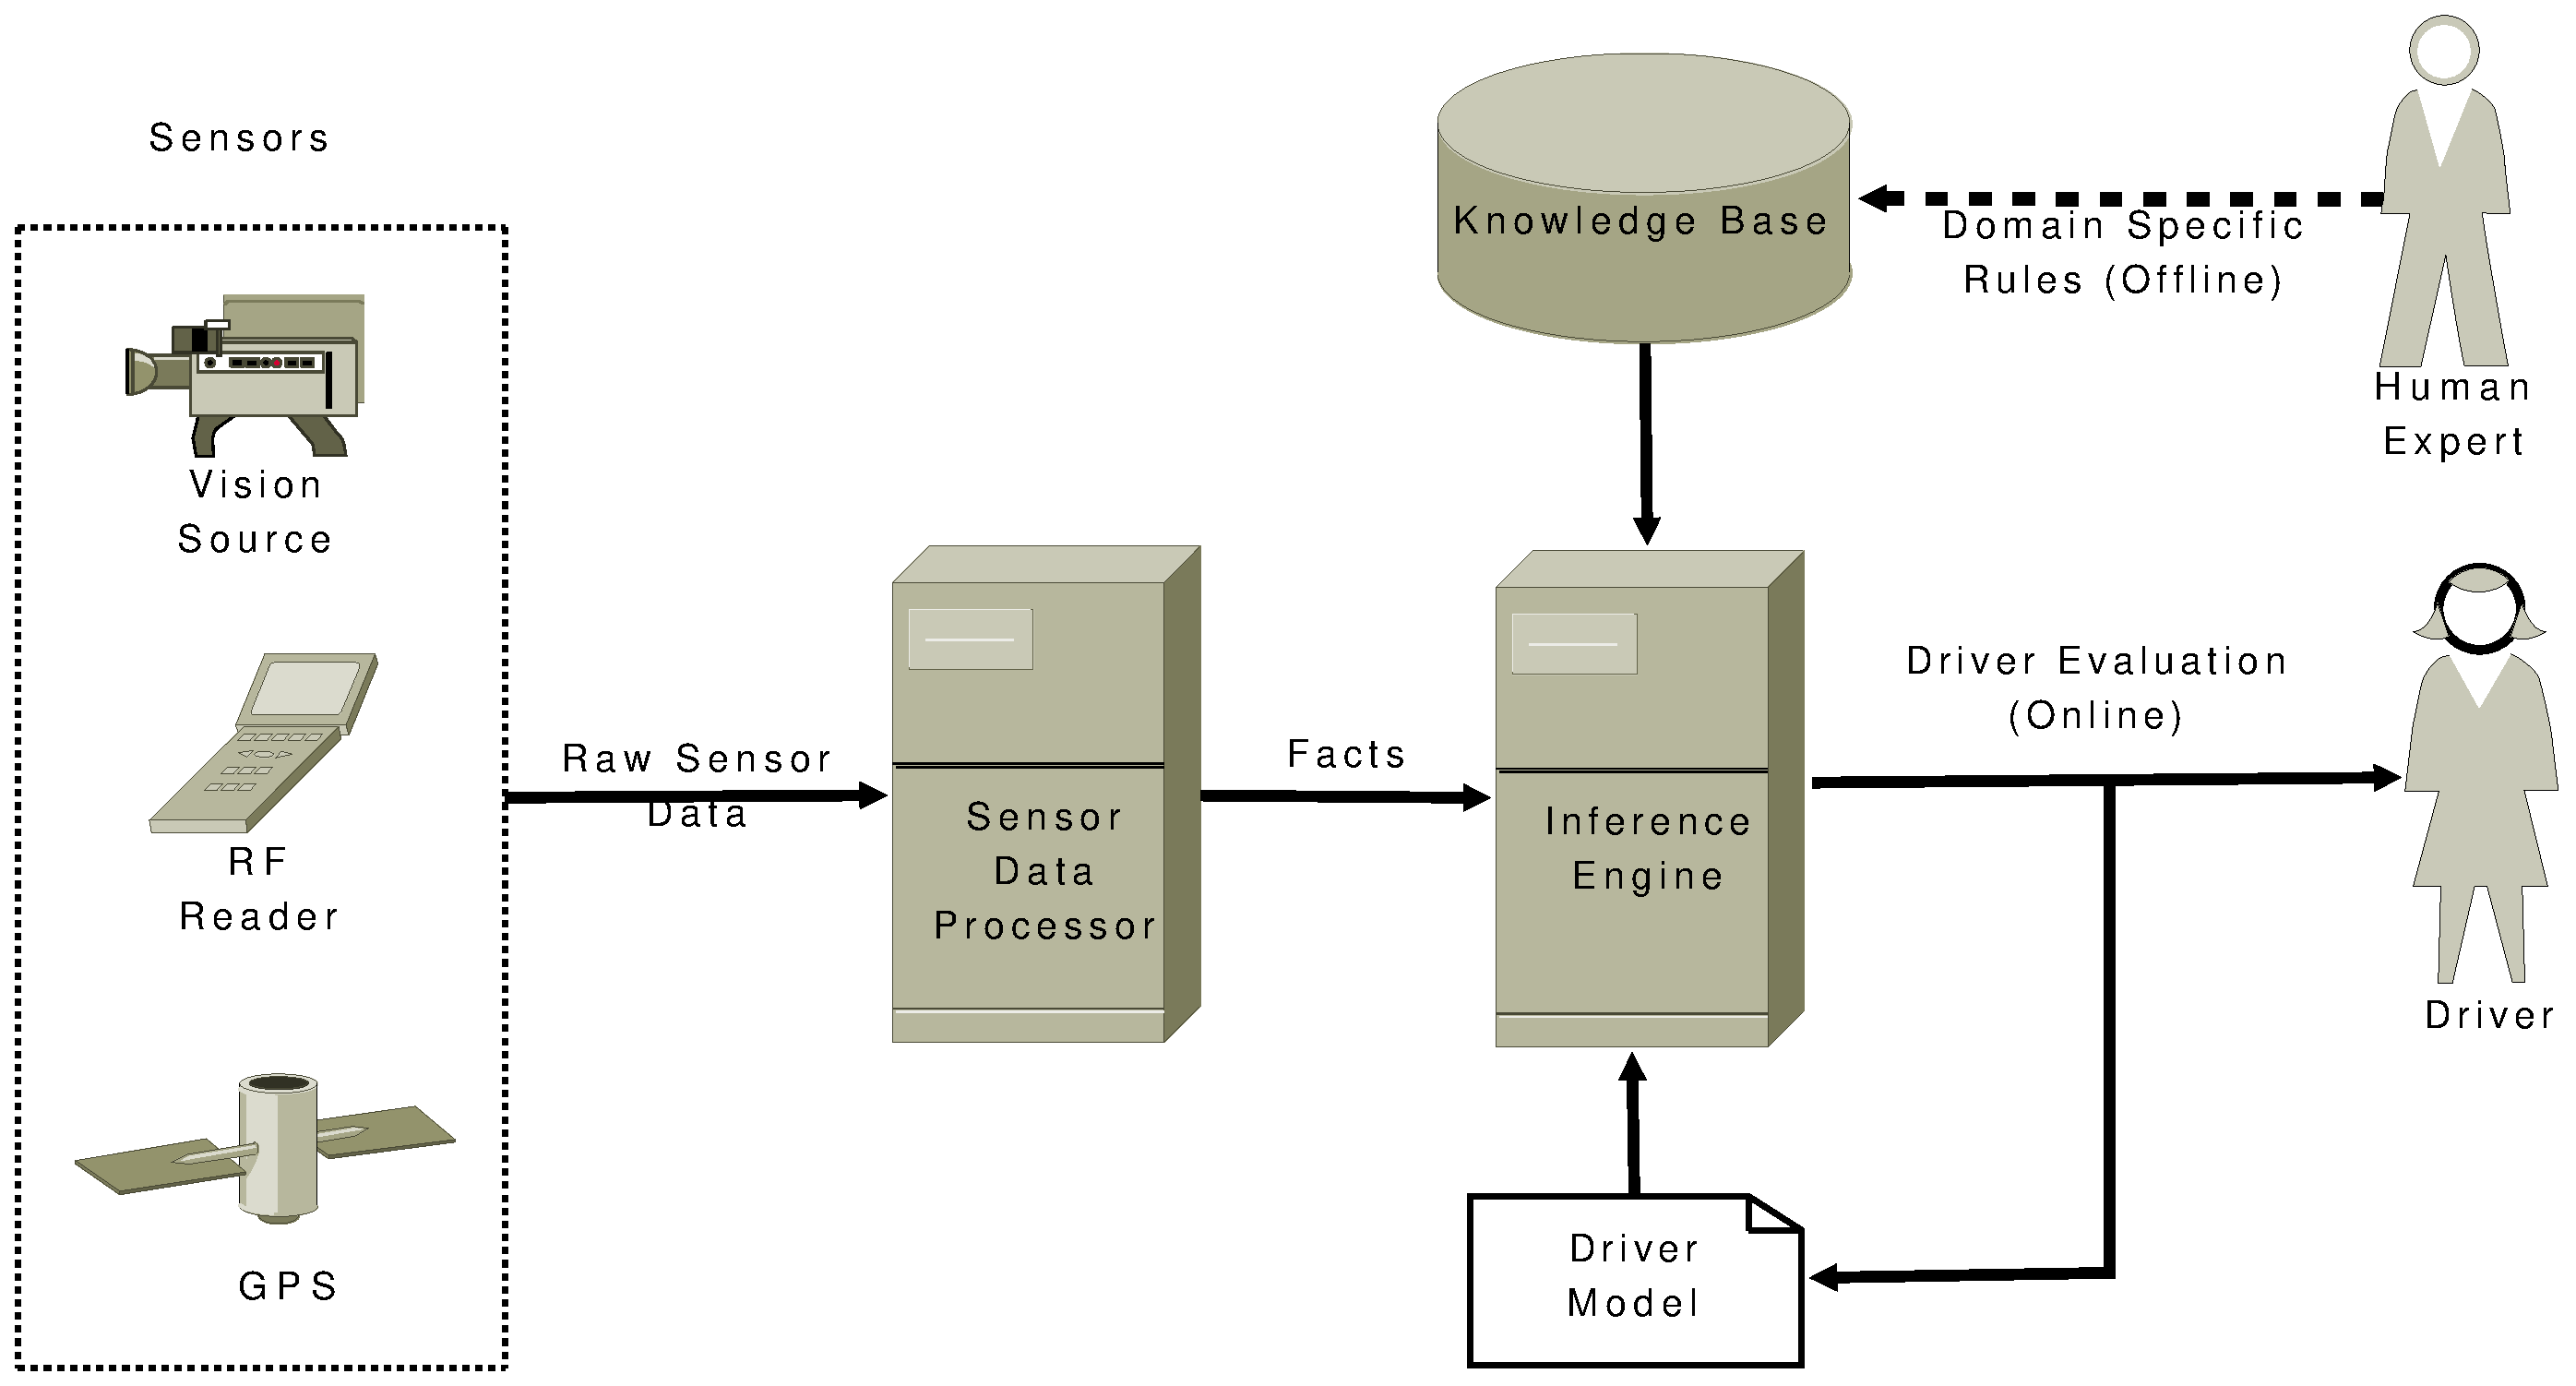
\includegraphics[width=70mm,height=35mm]{img/sys3.eps}
\caption{Basic system architecture of ADES project.}
\label{fig:sys}
\end{center}
\end{figure}
\par

The proposed approach for sign detection and classification can be divided into three stages:
\begin{itemize}
	\item \textbf{Preprocessing Stage:} Brightness of the image is normalized.
	\item \textbf{Sign Detection Stage:} Traffic signs in the image are detected.
	\item \textbf{Classification Stage:} The detected signs are classified into the known set of traffic signs. 
\end{itemize}


The set of images includes the known traffic signs shown in Figure \ref{fig:signs}. The circular ones are regulatory and the triangular ones are the warning signs in our country. The proposed approach benefits from the red borders which is the most distinct common property of these signs. However, the proposed detection method can be used for different traffic signs in other countries with appropriate fitness functions.

\begin{figure}[ht]
\begin{center}
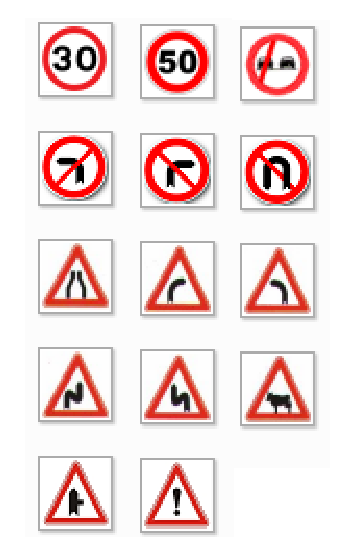
\includegraphics[width=30mm,height=50mm]{img/signs.eps}
\caption{Traffic signs recognized by the proposed system.}
\label{fig:signs}
\end{center}
\end{figure}
\par

\subsection{Adaptive Brightness Correction}
Although there are numerous advanced brightness correction techniques ~\cite{chen03, yang08}, we propose two simple brightness correction methods for improving the performance of image processing, which can be implemented for real-time applications. Both methods try to differentiate the red regions of the image by assigning the most proper values for the parameters $\alpha$ and $\beta$ introduced in the following equation.
\begin{eqnarray}
\label{eq1}
f(r,g,b)&=& \left\{\begin{array}{l} 1, r>\alpha \times g, r>\beta \times b \\ 0, o/w \end{array} \right.
\end{eqnarray}

\noindent where $r$, $g$ and $b$ are the red, green, and blue components of a pixel.
 
\subsubsection{Mean based brightness adaptation}
The mean based brightness adaptation approach uses histograms of the acquired frame. Sample scenes with corresponding red, green, blue histograms are given in Figure \ref{fig:hist1}. The values of $\alpha$ and $\beta$ in Equation \ref{eq1} are calculated according to Equation \ref{eq2} where $HSL$ denote the hue, saturation and lightness histogram arrays.

\begin{eqnarray}
\label{eq2}
HIST &=& Histogram(HSL_{rgb}) \\
\nonumber \alpha = \beta &=& 1 + L_{mean}/2
\end{eqnarray}

\begin{figure}[H]
\begin{center}
\includegraphics[width=70mm,height=60mm]{img/hist1.eps}
\caption{Good, medium and poor conditions for traffic sign detection.}
\label{fig:hist1}
\end{center}
\end{figure}

\subsubsection{Selected point count based brightness adaptation}
In the selected point count based brightness adaptation approach, the parameter values are adjusted according to the total number of white pixels in the binarized image. If the number of the white pixels is less than a threshold then the parameters are slightly relaxed. On the other hand, if there are too many white pixels, then the parameters are tightened. The transformation is given by Equation \ref{eq3}.

\begin{eqnarray}
\label{eq3}
p_{i} &=& \left\{\begin{array}{l} 1, p=white \\ 0, p=black \end{array} \right.\\
\nonumber p_{white} &=& \sum{p_{i}}, \forall p \in image \\
\nonumber \alpha &=& \left\{\begin{array}{l} \alpha \times \alpha', p_{white}>max_{white} \\ \alpha/\alpha', p_{white}<min_{white} \\ \alpha, o/w \end{array} \right.\\
\nonumber \alpha' &>& 1\\
\nonumber \beta &=& \left\{\begin{array}{l} \beta \times \beta', p_{white}>max_{white} \\ \beta/\beta', p_{white}<min_{white} \\ \beta, o/w \end{array} \right.\\
\nonumber \beta' &>& 1
\end{eqnarray}

\noindent where $p$ is a pixel on the binarized image. The values of $\alpha'$ and $\beta'$ are usually assigned slightly higher than one (e.g 1.05) to prevent major changes in the consecutive frames. However, the effect of the adaptation is not reduced because of the high frame rate of the streaming media. In Figure \ref{fig:adapbright} the sign becomes clearer as the $\alpha$ and $\beta$ values become 1.02, 1.04, and 1.104 respectively.

\begin{figure}[H]
\begin{center}
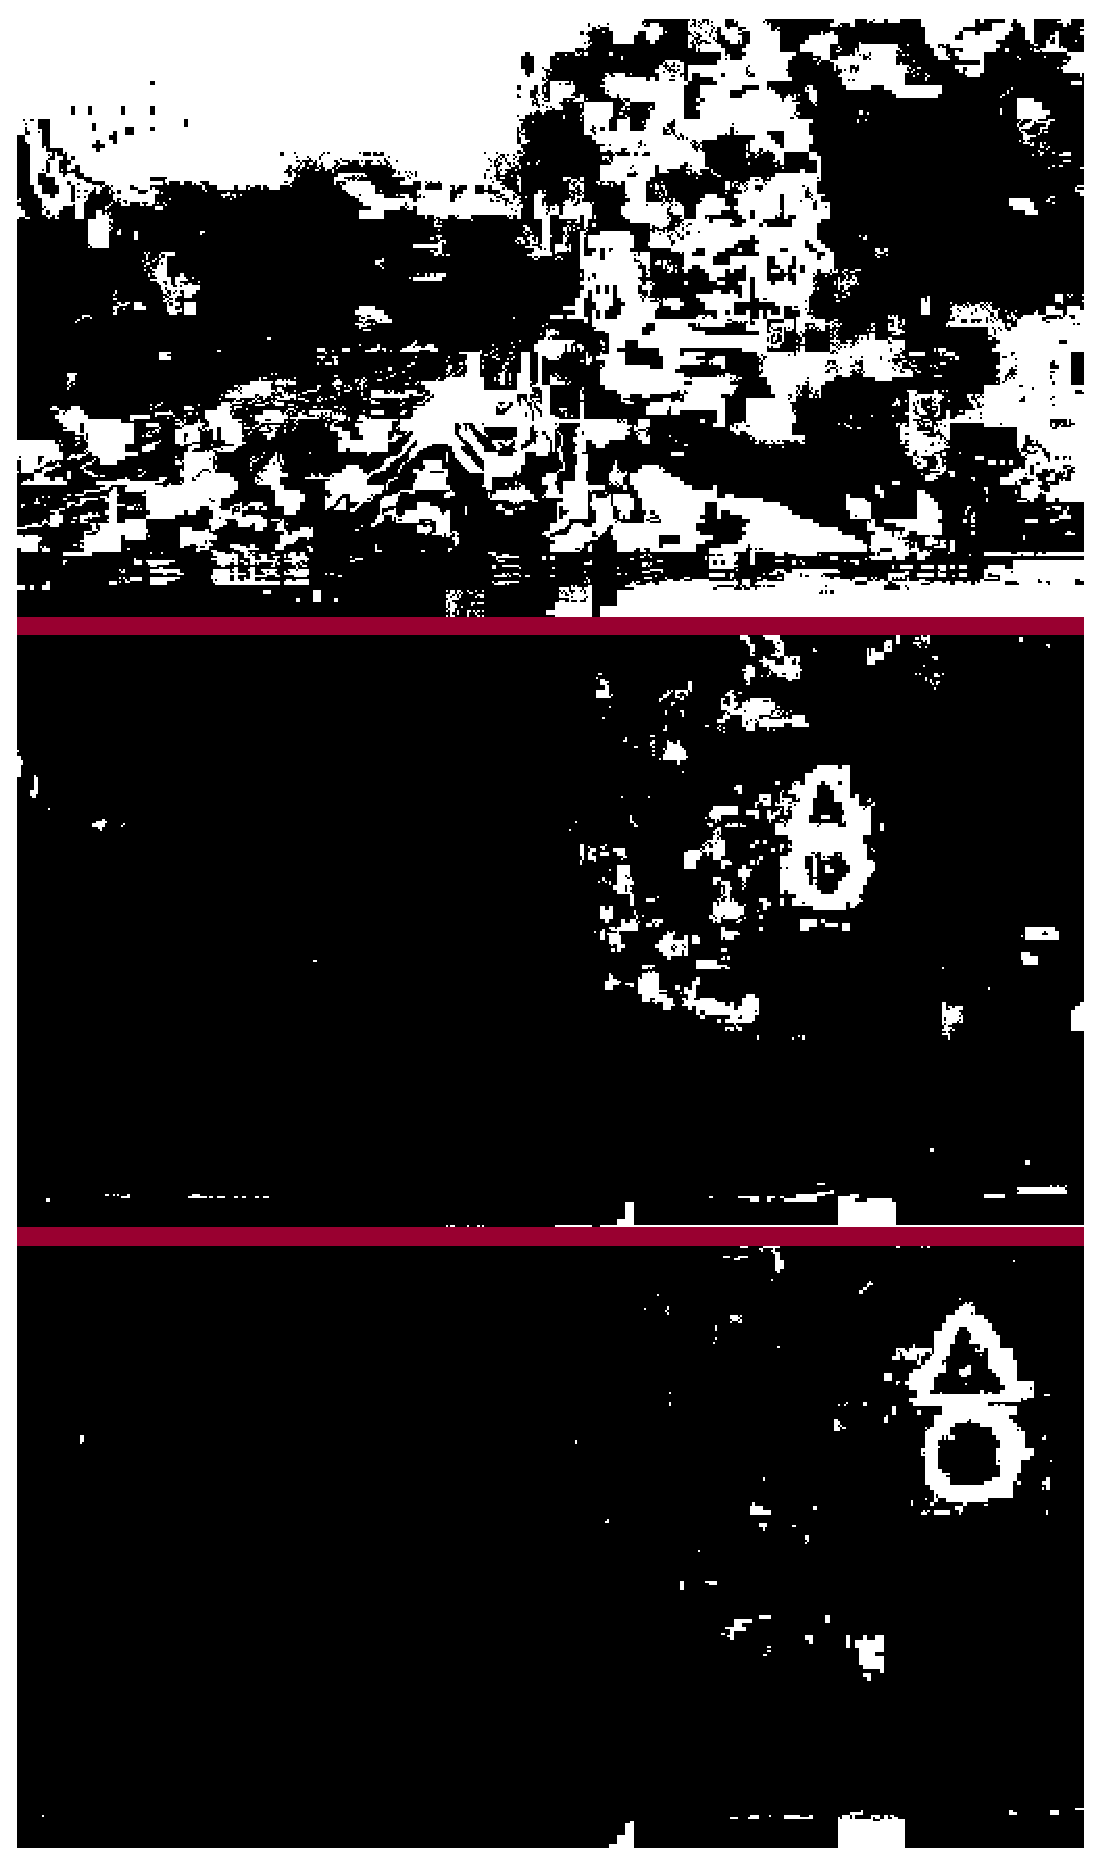
\includegraphics[width=40mm,height=60mm]{img/adapbright.eps}
\caption{Effect of brightness adaptation on image binarization.}
\label{fig:adapbright}
\end{center}
\end{figure}

\subsection{Sign Detection}
The proposed approach for sign detection and tracking is based on genetic algorithms (GA) \cite{miscbib05}. The GA process benefits from a modified version of radial symmetric transform \cite{signbib26}. 

\subsubsection{GA Process}

\paragraph{Encoding}
The GA implementation proposed by this study uses the coefficients of an affine transformation applied to a set of points describing the characteristics of a given template. The geometric transformation, which includes affine and perspective transformations, is
\begin{eqnarray}
\label{eq4}
\begin{bmatrix}
  u'\\
  v'\\
  w
\end{bmatrix}
&=&
\begin{bmatrix}
  a & b & c\\
  d & e & f\\
  g & h & 1
\end{bmatrix}
\begin{bmatrix}
  x\\
  y\\
  1
\end{bmatrix}\\
\nonumber u &=& u'/w \\
\nonumber v &=& v'/w
\end{eqnarray}
\noindent where $x$ and $y$ are the coordinates of the sample point from the template describing the set of points. $u$ and $v$ are the transformed points on the image. $a$, $b$, $d$, $e$ provide rotation, scaling and shearing, and $c$ and $f$ are used for translation. In addition, $g$ and $h$ provide perspective transformation in two dimensions. These coefficient values or a subset of them can be used in the chromosome encoding of the GA.

The effect of the transformation can be visualized better with a simple example. Assume that $a$, $b$, $c$, $d$, $e$, and $f$ coefficients are used in the encoding of the GA chromosome. In addition, $g$ and $h$ are assumed to be zero since the perspective transformation is beyond the scope of this study. For this scenario, we can conclude that a chromosome with the transformation coefficients in Equation \ref{eq5} can yield the transformed circle and triangular points shown in Figure \ref{signfig07}. The points on the left hand side of each figure are the equidistant characteristic points of the circular and triangular templates, where the points on the right hand sides are the translated, scaled, and rotated counter parts in the transformed domain.
\begin{eqnarray}
\label{eq5}
\begin{bmatrix}
  u\\
  v\\
  1
\end{bmatrix}
&=&
\begin{bmatrix}
  2 & 1 & 100\\
  1 & 2 &  50\\
  0 & 0 &   1
\end{bmatrix}
\begin{bmatrix}
  x\\
  y\\
  1
\end{bmatrix}
\end{eqnarray}

\begin{figure}[H]
\begin{center}
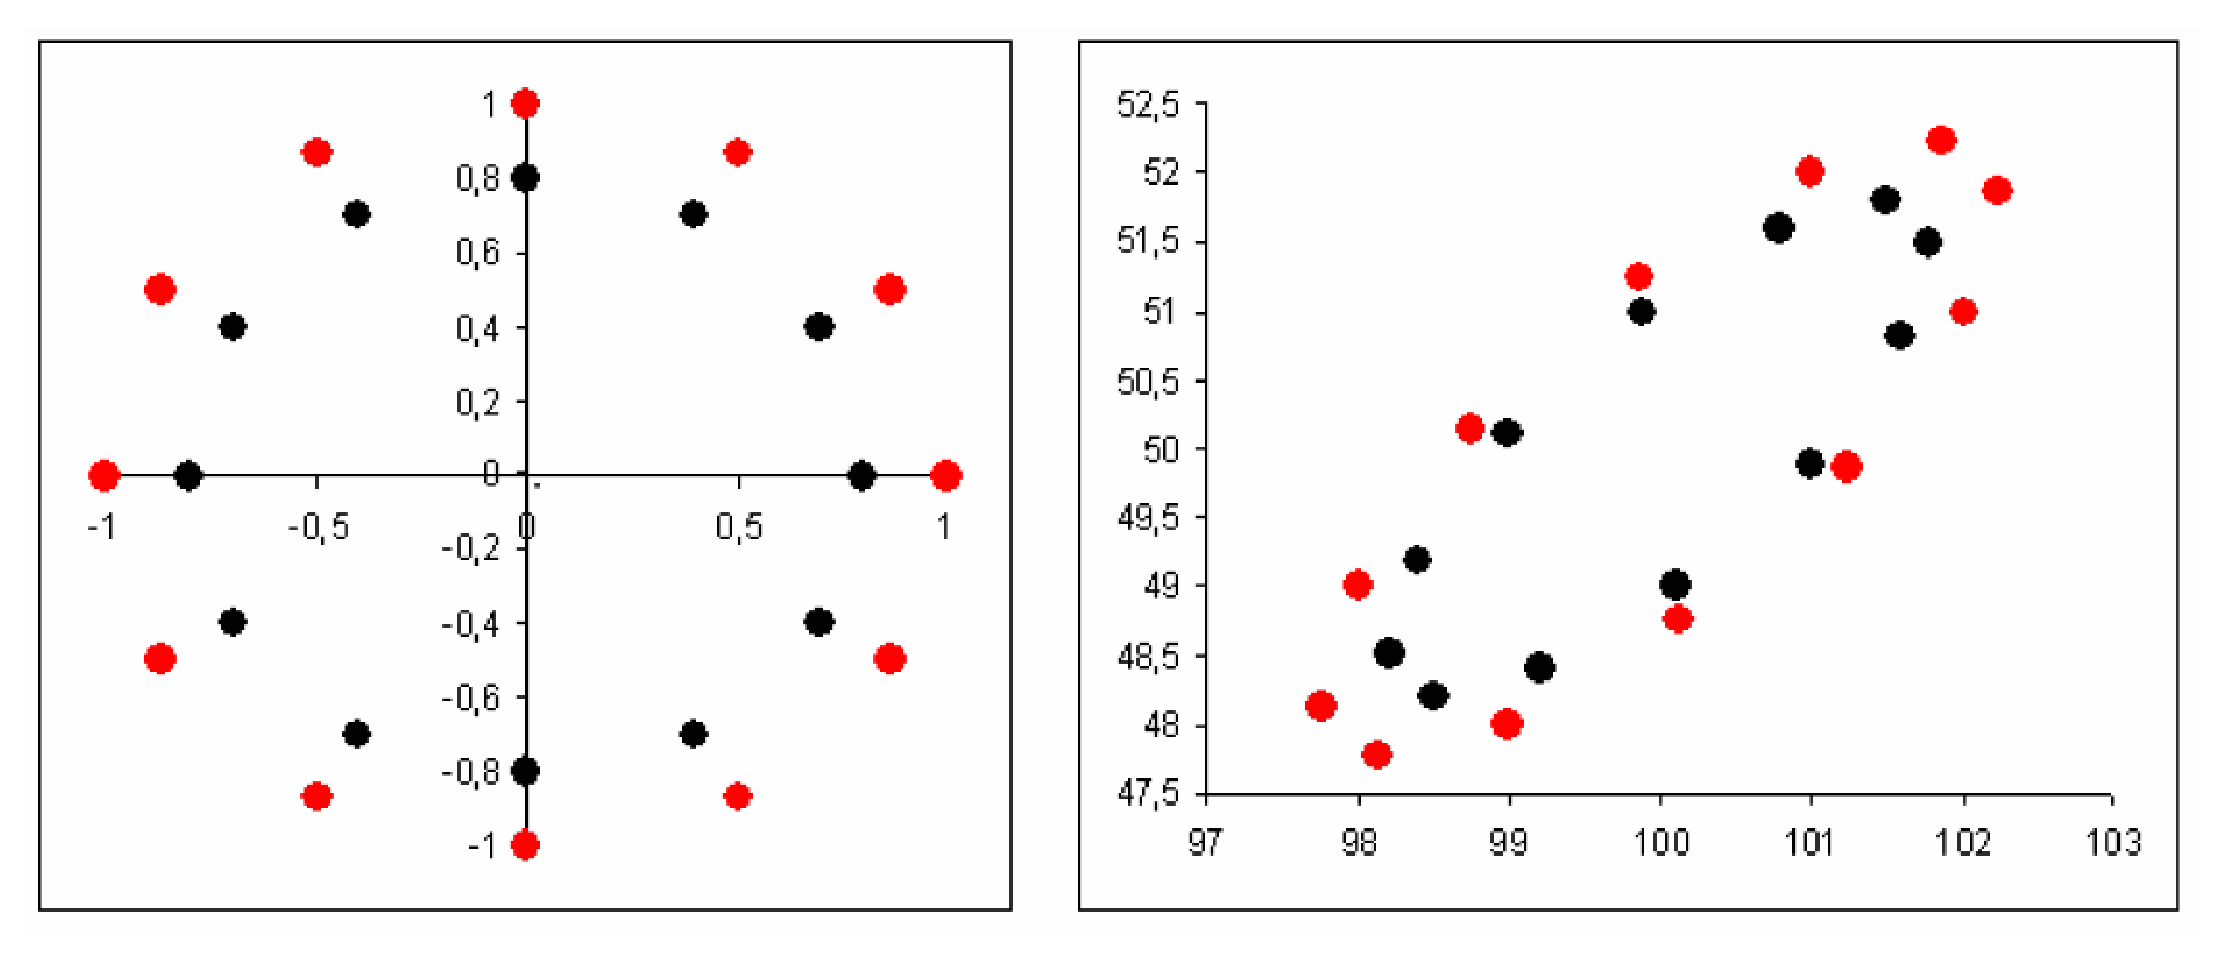
\includegraphics[scale=0.17]{img/signfig06.eps}\\
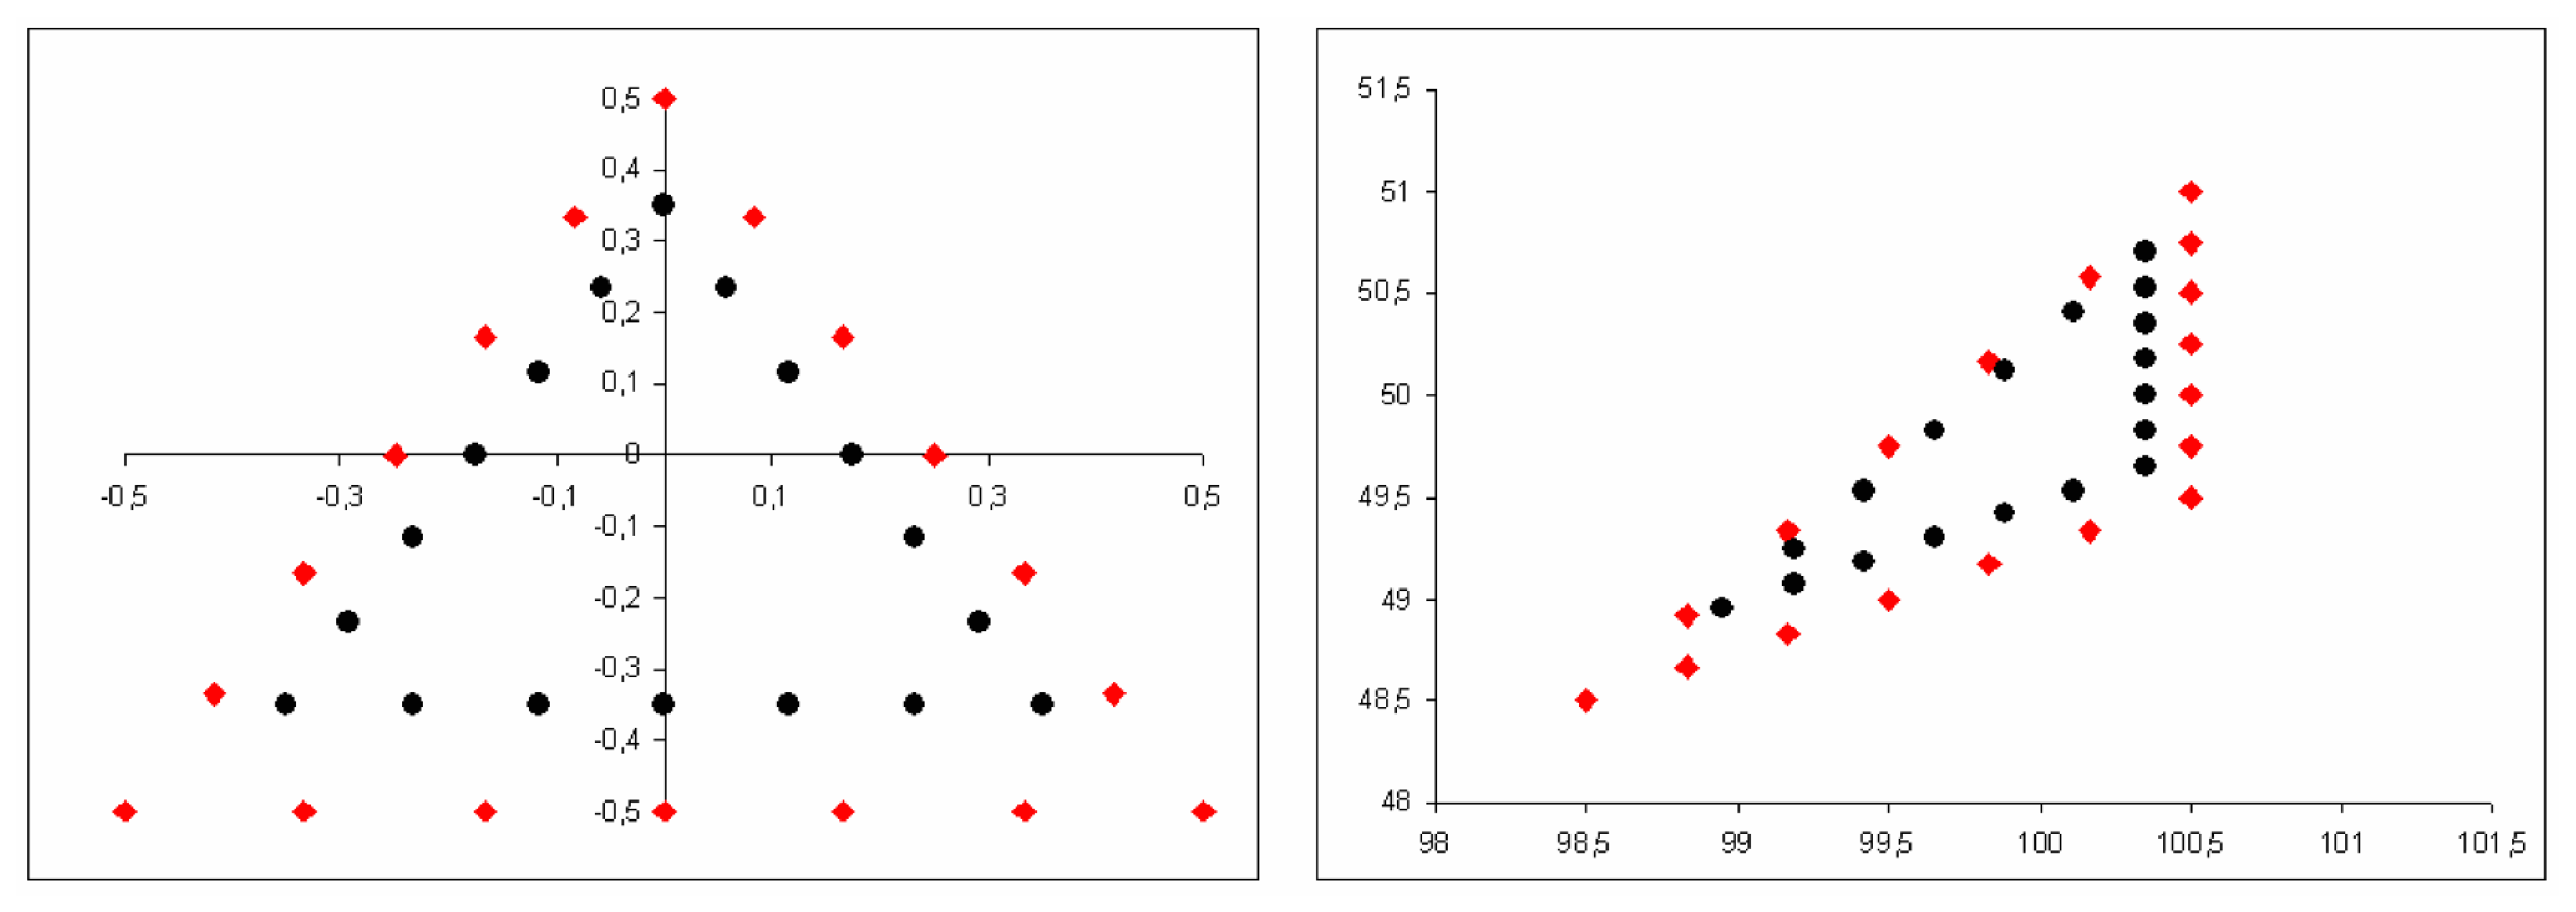
\includegraphics[scale=0.13]{img/signfig07.eps}
\caption{Template characteristic points in $(x, y)$ domain, and $(u, v)$ domain after affine transformation for circular and triangular signs.}
\label{signfig07}
\end{center}
\end{figure}

For complex applications, all of the geometric transformation matrix values can be added to the chromosome encoding in the same manner, however, the resulting search space may not be convenient for real time applications in case of limited computational power. Therefore, in this particular study, only the two translation and one scaling coefficients are included in the chromosome in order to reduce the computational requirements. The shearing and rotation can be introduced to the solution by providing feasible limits for $b$, $d$, $e$ coefficients. A similar crossover operation can also be defined for those parameters. But these parameters are ignored in this study for simplicity. The resulting transition matrix is given in Equation \ref{eq6}.

\begin{eqnarray}
\label{eq6}
\begin{bmatrix}
  u\\
  v\\
  1
\end{bmatrix}
&=&
\begin{bmatrix}
  a & 0 & c\\
  0 & a & f\\
  0 & 0 & 1
\end{bmatrix}
\begin{bmatrix}
  x\\
  y\\
  1
\end{bmatrix}
\end{eqnarray}

\paragraph{Crossover Operator}
The crossover process is also a function of affine transformation coefficients as given in Equation \ref{eq7}
\begin{eqnarray}
\label{eq7}
\nonumber a_{newchromo}&=&\eta a_{chromo1}+\mu a_{chromo2} \\
c_{newchromo}&=&\eta c_{chromo1}+\mu c_{chromo2} \\
\nonumber f_{newchromo}&=&\eta f_{chromo1}+\mu f_{chromo2} \\
\nonumber  \eta+\mu &=& 1
\end{eqnarray}
\par

\paragraph{Fitness Evaluation}
The fitness of the chromosome is evaluated according to the color of the transformed point $(u,v)$ on the binary image. If the value of the pixel is one, which means it is a red point on the original image, the fitness of the chromosome is increased. Obviously, this method would yield the highest fitness value for completely red regions. Therefore another set of template points is used to consider the non-red points on the template. These points are also subject to the transformation. These non-red points are selected inside the region bounded by the red points as shown in Figure \ref{signfig07}. In other words, the red points increase the fitness value when they are white in the binary image, and the black points increase the fitness value when they are black in the binary image. If the expected color cannot be found, then the fitness value is decreased for each of the failed points. At each iteration, the fitness values are calculated for each chromosome. At the end of the process the chromosomes are expected to converge around the traffic sign as shown in Figure \ref{signfig09}.
\begin{figure}[H]
\begin{center}
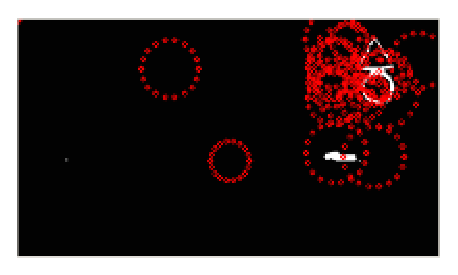
\includegraphics[scale=0.5]{img/signfig08.eps}

\includegraphics[scale=0.5]{img/signfig09.eps}
\caption{Initial and converged chromosomes.}
\label{signfig09}
\end{center}
\end{figure}
\par
Half of the converged chromosomes in each frame are used in the evaluation of the next frame. This approach has two benefits. First, the tracking of the detected signs can be achieved by using the transferred chromosomes. And second, since the consecutive simulations are not independent, the number of generations for the GA simulation can be reduced considerably.

\subsubsection{Modified Radial Symmetry Check}

After the GA process, an additional step of \textsl{Modified Radial Symmetry} check is introduced for tuning the position of the sign. This process also works as a sanity check for the detected region.

\par
\paragraph{Circular Sign Case}
For the circular sign detection, this check works as shown in Figure \ref{signfig10}(a). The "Start" point is the outcome of the GA process. For each candidate point suggested by the GA process, the \textit{Circle Validation Algorithm} detects the innermost circle that surrounds the point. First, the algorithm performs a bi-directional horizontal scan, and finds the $x$-coordinate center (Center $\sharp$1). The vertical center is detected next, by performing a bi-directional vertical scan starting from Center $\sharp$1. Note that, this is the simplified description of the algorithm. In the actual implementation, the algorithm employs a probabilistic approach, and detects the maximum of 2$^\textit{N}$ x 2$^\textit{N}$ candidate circles, where \textit{N} is the tolerance coefficient. This coefficient \textit{N} enables tolerating the discontinuities on the circle.

\begin{figure}[ht]
\begin{center}
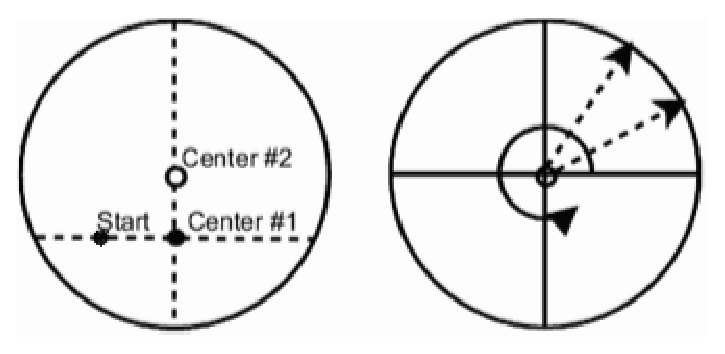
\includegraphics[scale=0.5]{img/signfig10.eps}
\caption{(a) Circle detection, (b) Scoring of circles.}
\label{signfig10}
\end{center}
\end{figure}
\par
After the detection step, each candidate circle is scored as displayed in Figure \ref{signfig10}(b). The scoring function projects the virtual circle onto the binarized image. Next, a scoring function checks how good the candidate circle overlaps with the red points in the binarized image. If the candidate circle really overlaps a circle on the actual image, it will get a high score (Figure \ref{signfig11}). This overlapping check is performed for $36$ points (10$^{\circ}$ increment) in our implementation. Hence the maximum score is $36$.
\par
\begin{figure}[ht]
\begin{center}
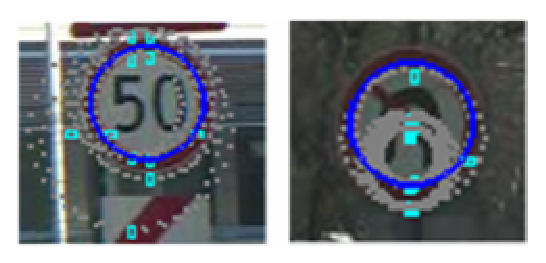
\includegraphics[scale=0.5]{img/signfig11.eps}
\caption{Candidate circles, and highest score selection.}
\label{signfig11}
\end{center}
\end{figure}
\par
\paragraph{Triangular Sign Case}
Triangular sign validation runs in a slightly different manner. As shown in Figure \ref{signfig14}(a), the detection phase is similar to that of the circular signs, but scoring is completely different. The difference in the geometry affects the Center $\sharp$2 location, which is \textit{radius}/3 upwards from the triangle baseline. Similar to the circular case, the algorithm detects the maximum of 2$^\textit{N}$ x 2$^\textit{N}$ candidate triangles, where $\textit{N}$ is the tolerance coefficient. 
\begin{figure}[ht]
\begin{center}
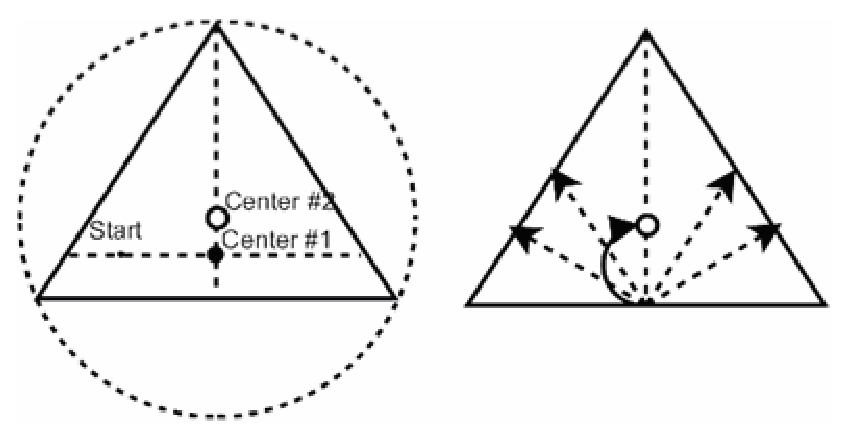
\includegraphics[scale=0.5]{img/signfig14.eps}
\caption{Candidate triangles, and highest score selection.}
\label{signfig14}
\end{center}
\end{figure}
\par
After the detection step, each candidate triangle is scored as displayed in Figure \ref{signfig14}(b). The center of the bottom edge is used as the reference point, since it is computationally favorable to deal with right angles. The maximum score a candidate triangle can get is $3 \times 9 = 27$ for the triangular case. 

In Figure \ref{signfig13} the detected signs are marked. Since the radial symmetry check provides information about the boundaries of the detected sign, the region within the boundaries is provided for sign classification phase.
\begin{figure}[ht]
\begin{center}
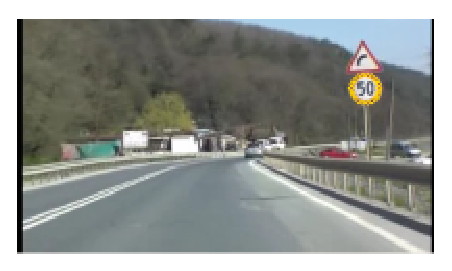
\includegraphics[scale=0.90]{img/signfig12.eps}
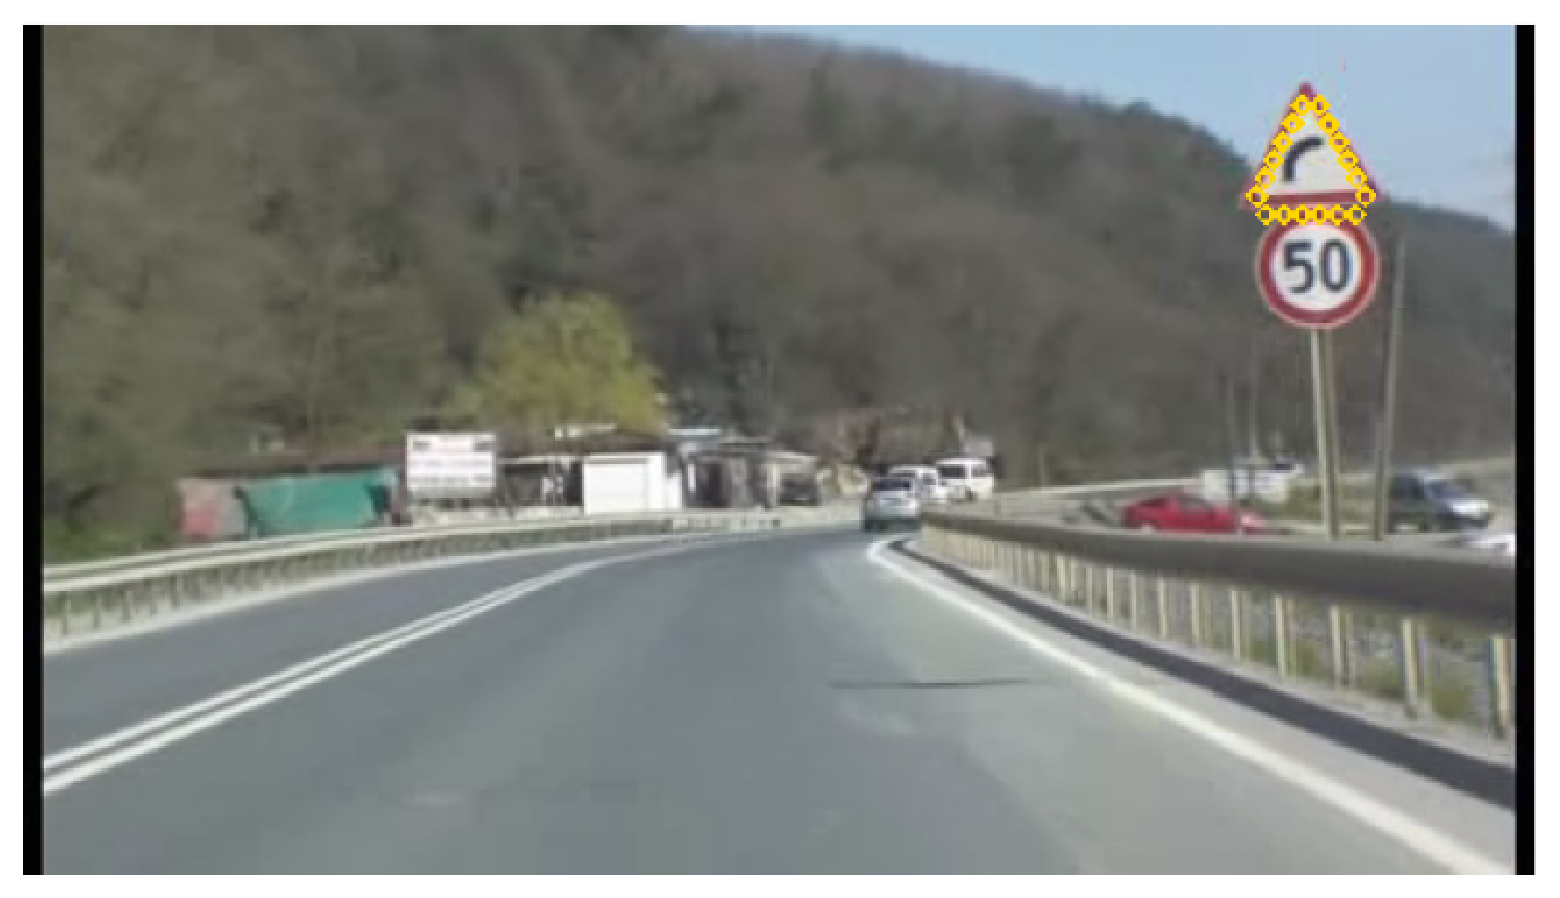
\includegraphics[scale=0.25]{img/signfig13.eps}
\caption{Detected traffic signs.}
\label{signfig13}
\end{center}
\end{figure}
\par

\subsection{Sign Classification}

The sign detection process explained in the previous section finds binary images resized to $64 \times 64$ pixels that contain the interior part of the traffic signs isolated from the red borders. These are human readable images but still need to be classified and mapped into a predefined set of signs. In order to perform classification, we first extract features, then use these features to classify the detected signs. We consider neural networks and support vector machines for classification.

\subsubsection{Feature Extraction}
As shown in Figure \ref{signfig27}, the detection output may not always be centered. In the majority of the cases, the center of mass (CoM) (identified by light blue) will not overlap the center of the $64 \times 64$ image (identified by red color). Therefore the CoM of the detected sign is calculated first and then this information is used for both of the considered feature extraction schemes as explained in the corresponding sections. The general idea about using CoM is to crop a smaller region of interest around the CoM for the feature extraction methods to process.
\begin{figure}[ht]
\begin{center}
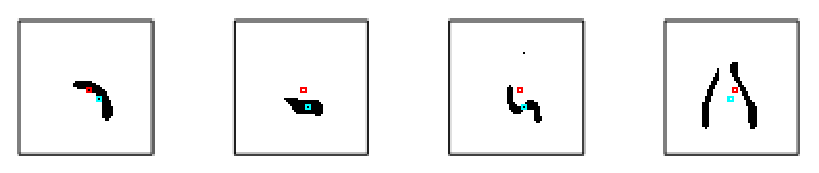
\includegraphics[scale=0.6]{img/signfig27.eps}
\caption{Deviation of CoM from image center.}
\label{signfig27}
\end{center}
\end{figure}
Our feature extraction method is similar to that of \cite{signbib02,Maldonadobascon07}. Escalera \textit{et al} \cite{signbib02} used $30 \times 30$ inputs to train neural networks. Maldonado-Bascon \textit{et al} \cite{Maldonadobascon07} detected $31 \times 31$ blocks in grayscale and only used a subset of the pixels, (what they called "pixels of interest") for training the SVM classifier. Our contribution is to use the CoM to better focus the signs, hence making the system invariant to translation. Resizing the innermost $24 \times 24$ image to $12 \times 12$ size further reduces the size of the input vectors for NN and SVM training.

\subsubsection{Classification}
After the detection process, the detected sign is serialized to a binary input array where each item is an input for the classifier. Two machine learning techniques are applied for sign classification.

\textit{NN-Based Classification:} In the current implementation, each traffic sign has its own feedforward neural network. In other words, a separate network with 4 hidden nodes and one output is trained for each sign. All the neurons have sigmoid activation functions. The networks are trained by using Levenberg-Marquardt learning technique \cite{wilamowski1999efficient}.

\textit{SVM Implementation:}SVM \cite{cortes1995support} models were originally defined for the classification of linearly separable classes of objects. The solution of the classification problem is a weighted sum of kernel functions evaluated at the support vectors. In our implementation, we used the same input values as explained in the previous section to train the SVM with the radial basis kernel function (RBF) given in Equation \ref{eq9}.
\begin{eqnarray}
\label{eq9}
	k(u,v) &=& e^{-\gamma \times |u-v|^2}
\end{eqnarray}
\noindent
where $k$ is the kernel function which gives the distance between the support vector $u$ and the test point $v$. The coefficient $\gamma$ is found by trying sample values at different exponential scales.

\section{Experiments and Results}
\label{sec:er}

\subsection{Experimental Setup}

The experiments are performed with a pre-recorded video sequence of 512 $\times$ 288 pixels resolution at 20 fps frame rate. Video capturing is done in a car moving with varying speed in actual urban traffic as shown in Figure \ref{signfig30}. A wide range of lighting conditions are included in the test videos. Sunny roads, dim lighted roads, shadows and even night-time driving conditions are considered.

\begin{figure}[ht]
\begin{center}
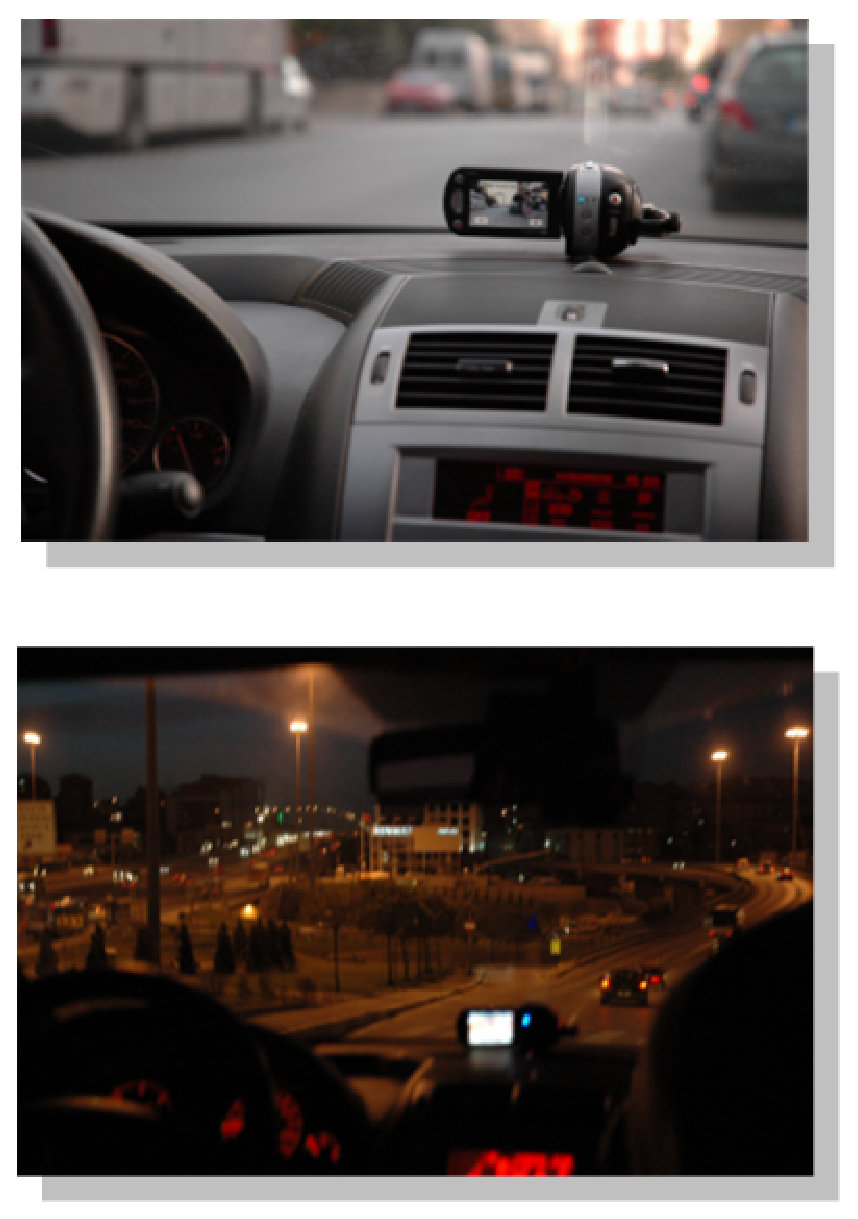
\includegraphics[scale=0.4]{img/signfig30.eps}
\caption{Video capturing setup. Day and night scenes.}
\label{signfig30}
\end{center}
\end{figure}

Video processing is performed on a PC with Intel T5450 processor at 1.66 GHz. Since the sign detection process should be carried out in real-time, we tried to keep the GA population and the number of iterations small. Besides, we used \textit{N}=2 as the tolerance coefficient for the \textit{Modified Radial Symmetry} step. This allows second level of discontinuity in any of the four directions while assuring a reasonable processing time.

\subsection{Detection Phase Results}

For the detection phase, we have done several measurements and obtained the results given in Tables \ref{signdetect-table-1} and \ref{signdetect-table-2}. The results show almost perfect CPU time utilization. For a highly acceptable detection process, 9 ms of CPU time is enough. Therefore, it is possible to re-run the whole process more than one hundred times in a second. This gives an opportunity to utilize the GA to track the detected sign over a sequence of frames. For this purpose, half of the best chromosomes at the end of each processed frame are passed to the next frame. 
\par
\begin{table}[ht]
	\centering
	\caption{Detection rate of circular signs.}
	\label{signdetect-table-1}
	\begin{tabular}{l r r r r}
		\hline
		\textbf{Fitness threshold} 		& 30 & 30 & 30 & 35 \\
		\textbf{Population size} 			& 60 & 120 & 60 & 60 \\
		\textbf{Number of Generations} 	& 2 & 2 & 4 & 2 \\
		\textbf{Mutation rate}     		& 0.35 & 0.35 & 0.35 & 0.35 \\
		\textbf{Crossover rate} 				& 0.75 & 0.75 & 0.75 & 0.75 \\
		\textbf{Selection method} 				& Elitist & Elitist & Elitist & Elitist \\
		\hline
		\rowcolor[rgb]{0.95,0.95,0.95}\textbf{Avg. Process Time(msec)}	& 9 & 14 & 14 & 9 \\
		\rowcolor[rgb]{0.95,0.95,0.95}\textbf{True detections (percent)} &  95 &  96 &  96 &  65 \\
		\rowcolor[rgb]{0.95,0.95,0.95}\textbf{Misses (percent)}	&  5 &  4 &  4 &  35 \\
		\hline
		\rowcolor[rgb]{0.95,0.95,0.95}\textbf{False detections (percent)}				&  5 &  7 &  6 &  1 \\
		\hline
	\end{tabular}
\end{table}
\par
The upper rows of the Tables \ref{signdetect-table-1} and \ref{signdetect-table-2} show the parameter sets, while the lower rows (painted in gray) show the experiment results. \textit{True detections} correspond to the correctly detected signs, whereas the \textit{misses} are the signs that could not be detected at all. Note that, the sum of true detections and misses is always 100 percent. \textit{False detections}, on the other hand, are the cases where the system indicates a sign existence even though there exists no sign in that location. \textit{False detection rate} is calculated by comparing the number of false detections with the total number of real traffic signs in the video. The first column of values in the tables, is the preferred set of parameters for both the circular and the triangular cases. 
\par
For the circular signs, a fitness threshold of 30, GA population size of 60 and 2 generations yields the ideal results in terms of accuracy and CPU time. It is possible to enhance the accuracy up to 96 percent by increasing either the population size or the number of generations. But this will almost double the processing time for a very small accuracy enhancement, hence is not worth the trade-off. The fitness threshold, on the other hand, has considerable effect on the accuracy, as seen on the rightmost column.
\par
The triangular sign process yields the ideal results with a fitness threshold of 16. That is due to the different geometric characteristics of the triangular signs. The \textit{true detection} rate degrades from 95 percent to 87 percent. It is possible to increase this value by decreasing the fitness threshold from 16 to 12. But this has a side-effect of increasing the false detections from 4 percent to 9 percent.

\begin{table}[ht]
	\centering
	\caption{Detection rate of triangular signs.}
	\label{signdetect-table-2}
\begin{tabular}{l r r r r}
\hline
\textbf{Fitness threshold} 		& 16 & 16 & 16 & 12 \\
\textbf{Population size} 			& 60 & 150 & 60 & 60 \\
\textbf{Number of Generations} 	& 2 & 2 & 6 & 2 \\
\textbf{Mutation rate}     		& 0.35 & 0.35 & 0.35 & 0.35 \\
\textbf{Crossover rate} 				& 0.75 & 0.75 & 0.75 & 0.75 \\
\textbf{Selection method} 				& Elitist & Elitist & Elitist & Elitist \\
\hline
\rowcolor[rgb]{0.95,0.95,0.95}\textbf{Avg. Process Time(msec)}			& 9 & 16 & 14 & 9 \\
\rowcolor[rgb]{0.95,0.95,0.95}\textbf{True detections (percent)}				& 87 & 88 & 90 & 94 \\
\rowcolor[rgb]{0.95,0.95,0.95}\textbf{Misses (percent)}				&  13 & 12 & 10 & 6 \\
\hline
\rowcolor[rgb]{0.95,0.95,0.95}\textbf{False detections (percent)}				&  4 &  4 &  5 &  9 \\
\hline
\end{tabular}
\end{table}

\subsection{Classification Phase Results}

In the second phase, Tables \ref{signclassify-table-1} and \ref{signclassify-table-2} exhibit the classification results on \textit{"properly detected"} signs. 

\begin{table}[ht]
	\centering
	\caption{Classification success rate of circular signs.}
	\label{signclassify-table-1}
\begin{tabular}{l r r}
\hline
\textbf{Classification Method} & NN & SVM \\
\hline
\rowcolor[rgb]{0.95,0.95,0.95}\textbf{Avg. Process Time(msec)}			& 5 & 10 \\
\rowcolor[rgb]{0.95,0.95,0.95}\textbf{Error rate (percent)}				& 9 &  20 \\
\hline
\end{tabular}
\end{table}
\begin{table}[ht]
	\centering
	\caption{Classification success rate of triangular signs.}
	\label{signclassify-table-2}
\begin{tabular}{l r r}
\hline
\textbf{Classification Method} & NN  & SVM  \\
\hline
\rowcolor[rgb]{0.95,0.95,0.95}\textbf{Avg. Process Time(msec)}			& 3 & 6 \\
\rowcolor[rgb]{0.95,0.95,0.95}\textbf{Error rate (percent)}				&  7 &  9 \\
\hline
\end{tabular}
\end{table}


\subsection{Overall System Performance}
\begin{table}[ht]
	\centering
	\caption{Overall system performance.}
	\label{signdetection-overall}
\begin{tabular}{|l|r r|}
\hline
& \multicolumn{2}{c|}{CIRCULAR} \\
\hline
\textbf{Classification Method} & NN & SVM \\
\hline
\textbf{Avg. Process Time(msec)}			& 14 & 19 \\
\hline
\textbf{Error rate (percent)}				&  14 &  24 \\
\hline

\hline
& \multicolumn{2}{c|}{TRIANGULAR} \\
\hline
\textbf{Classification Method} & NN & SVM \\
\hline
\textbf{Avg. Process Time(msec)}			& 12 & 15 \\
\hline
\textbf{Error rate (percent)}				&  11 &  13 \\
\hline
\end{tabular}
\end{table}

Table \ref{signdetection-overall} depicts the overall system performance, considering the detection and classification steps as a whole.  The errors of the detection step have an adverse effect on the classification process. For both circular and triangular signs, NN with $12 \times 12$ grid features have yielded the best results in terms of CPU time and error rate. The visual results of the experiments and the related data set can be found on the project web site \cite{miscbib04}.

\subsection{Comparison with Other Approaches}

The comparison of the overall system with the proposed systems in the last decade is given in Table \ref{tab:perf}. It can be seen that the overall accuracy of the system with NN classification is comparable if not better than the other approaches. Additionally,  the processing time of each frame is at least one order of magnitude smaller than any of the approaches even without considering the differences in the platforms.


\begin{sidewaystable}
\centering
\caption{Comparison of the Proposed Approach with selected methods from the last decade.}
\label{tab:perf}
\begin{tabular}{|p{19mm}|p{15mm}|l|l|r|r|r|}
\hline
{\bf Method} & {\bf Reference} & {\bf Year} & {\bf Hardware} & {\bf Image Size (px)} & {\bf Time (msec)} & {\bf Success Rate (\%)} \\
\hline
Matching Pursuit &        Hsu and Huang~\cite{signbib05}&       2000 &   Intel P2 &    512x480 &       ~250 &   up to 88 \\
\hline
Genetic Algorithm &   Escalera \textit{et al}~\cite{signbib10}&       2002 & AMD Duron 1Ghz &    384x286 & ~450 (51x8.8) &        N/A \\
\hline
Kalman Filter &       Fang \textit{et al}~\cite{Fang03}&       2003 & Intel P4 1GHz &    320x240 &      $>$1000 &        N/A \\
\hline
Feature Extraction &        Gao \textit{et al}~\cite{Gao2006}&       2005 &   Intel P3 &  1680x1680 &       ~450 &   up to 95 \\
\hline
       SVM &     Maldonado-Bascon \textit{et al}~\cite{Maldonadobascon07}&       2005 & Intel P4 2.2Ghz &    720x576 &      $>$ 1000 &   up to 93 \\
\hline
Geometric Fragmentation &   Soetedjo and Yamada~\cite{signbib11} &       2005 & Intel P4 2.6 GHz &    240x180 &       ~750 &   up to 86 \\
\hline
Haar Wavelet Features &   Bahlmann \textit{et al}~\cite{Bahlmann05}&       2005 & Intel Xeon 2.8Ghz &    384x288 &       ~100 &         85 \\
\hline
Neural Networks &      Nguwi and Kouzani~\cite{nguwi08}&       2006 & Pentium M 1.7Ghz &        N/A &       ~550 &   up to 95 \\
\hline
  Adaboost &       Baro \textit{et al}~\cite{baro09}&       2007 &        N/A & 60x60 stereo &      $>$ 1000 &      87-90 \\
\hline
Color Distance Transform &       Ruta \textit{et al}~\cite{signbib19}&       2007 &        N/A &    640x480 &        ~35 &   up to 85 \\
\hline
Affine Trans., GA, NN & Proposed Approach &       2010 & Intel T5450 1.66Ghz &    512x288 &        ~13 &         87 \\
\hline
\end{tabular}  
\end{sidewaystable}

\section{Conclusions}
\label{sec:conc}

This study proposes a real-time traffic sign detection, tracking, and classification system with several contributions to improve the different phases of sign detection and classification. The injection of affine transformation matrix into GA is the first novel contribution which makes the system immune to the rotation and the translation of the signs. Another contribution is the radial symmetry check for the GA output. This additional step provides better generations to the crossover operation. It acts like a sanity check for the fitness function and forms the basis of preventing false detections.

Using the proposed approach it is possible to process a frame on the average in 13 msec which is at least one order of magnitude smaller than any of the compared approaches even without considering the differences in the platforms. With NN classification, the overall accuracy of the system is also comparable if not better than the other approaches in the literature.  This shows that this system can be a part of a more complex real time application such as the proposed real time driver evaluation system.

Although only circular and triangular signs are considered in this study, the existing implementation can also process any kind of sign that can be described by a set of characteristic points. 

As a future work, we consider injecting more semantic rules into the system to increase the ability of the system to distinguish the sign candidate regions from the road, vehicles, sky and buildings in advance under more extreme conditions, so that brightness correction may only be applied to the candidate regions, thus helping to further reduce the error rate.


\bibliographystyle{model1-num-names}
\bibliography{journal}

\end{document}


